\begin{figure}[H]
    \centering

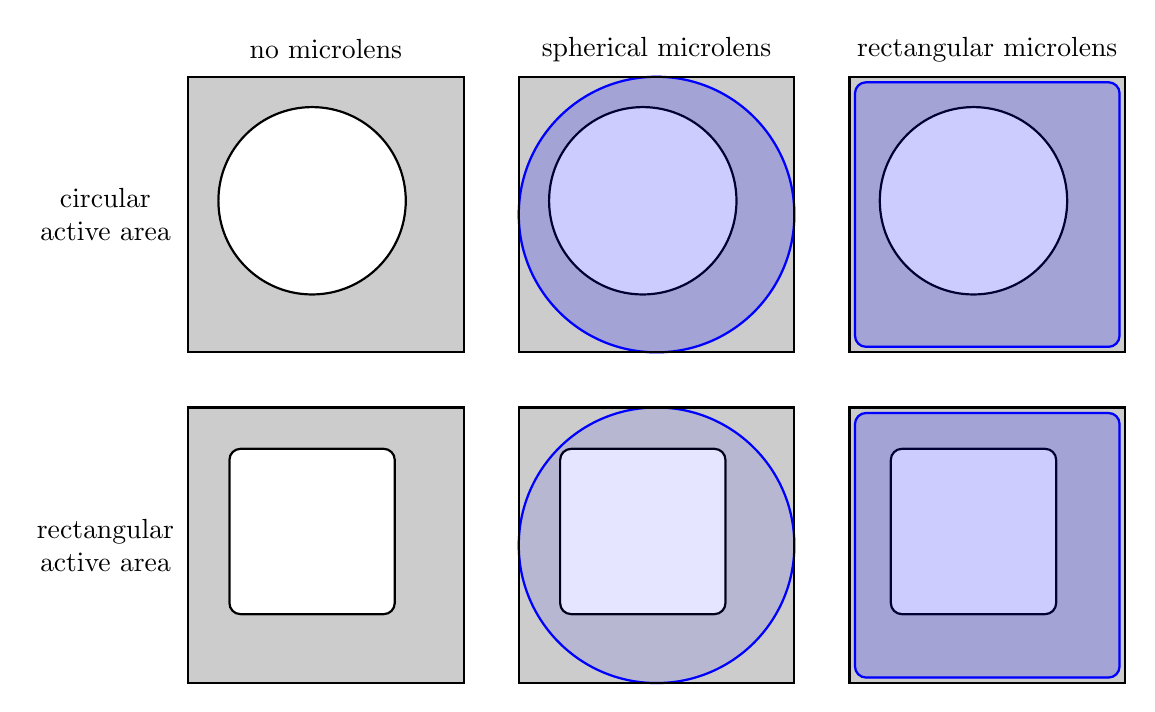
\begin{tikzpicture}[thick,scale=0.7, every node/.style={scale=1}]

\draw[fill, color=black!20]  (-2.5,3.5) rectangle (2.5,-1.5);
\draw[fill, color=white]  (-0.25,1.25) ellipse (1.7 and 1.7);
\draw[]  (-0.25,1.25) ellipse (1.7 and 1.7);

\draw[fill, color=black!20]  (3.5,3.5) rectangle (8.5,-1.5);
\draw[fill, color=white]  (5.75,1.25) ellipse (1.7 and 1.7);
\draw[]  (5.75,1.25) ellipse (1.7 and 1.7);
\draw [fill, color=blue, opacity=0.2] (6,1) ellipse (2.5 and 2.5);
\draw [color=blue] (6,1) ellipse (2.5 and 2.5);

\draw[fill, color=black!20]  (9.5,3.5) rectangle (14.5,-1.5);
\draw[fill, color=white]  (11.75,1.25) ellipse (1.7 and 1.7);
\draw[]  (11.75,1.25) ellipse (1.7 and 1.7);
\draw [fill, color=blue, opacity=0.2, rounded corners] (9.6,3.4) rectangle (14.4,-1.4);
\draw [color=blue, rounded corners] (9.6,3.4) rectangle (14.4,-1.4);

\draw[fill, color=black!20]  (-2.5,-2.5) rectangle (2.5,-7.5);
\draw[fill, color=white, rounded corners] (-1.75,-3.25) rectangle (1.25,-6.25) {};
\draw[rounded corners] (-1.75,-3.25) rectangle (1.25,-6.25) {};

\draw[fill, color=black!20]  (3.5,-2.5) rectangle (8.5,-7.5);
\draw[fill, color=white, rounded corners] (4.25,-3.25) rectangle (7.25,-6.25) {};
\draw[rounded corners] (4.25,-3.25) rectangle (7.25,-6.25) {};
\draw [fill, color=blue, opacity=0.1] (6,-5) ellipse (2.5 and 2.5);
\draw [color=blue] (6,-5) ellipse (2.5 and 2.5);

\draw[fill, color=black!20]  (9.5,-2.5) rectangle (14.5,-7.5);
\draw[fill, color=white, rounded corners] (10.25,-3.25) rectangle (13.25,-6.25) {};
\draw[rounded corners] (10.25,-3.25) rectangle (13.25,-6.25) {};
\draw [fill, color=blue, opacity=0.2, rounded corners] (9.6,-2.6) rectangle (14.4,-7.4);
\draw [color=blue, rounded corners] (9.6,-2.6) rectangle (14.4,-7.4);

\draw[]  (-2.5,3.5) rectangle (2.5,-1.5);
\draw[]  (3.5,3.5) rectangle (8.5,-1.5);
\draw[]  (9.5,3.5) rectangle (14.5,-1.5);

\draw[]  (-2.5,-2.5) rectangle (2.5,-7.5);
\draw[]  (3.5,-2.5) rectangle (8.5,-7.5);
\draw[]  (9.5,-2.5) rectangle (14.5,-7.5);

\node at (0,4) {no microlens};
\node at (6,4) {spherical microlens};
\node at (12,4) {rectangular microlens};
\node[align=center] at (-4,1) {circular\\active area};
\node[align=center] at (-4,-5) {rectangular\\active area};
\end{tikzpicture}
    \caption{Options for lenzes with varying types of active areas and microlenses}
    \label{tkz:SPAD_types}
\end{figure}